\section{Conduite de projet}
Pour réussir tout projet, il est indispensable de mettre en place une bonne méthodologie de travail. Une bonne méthodologie de travail est celle qui donne à une équipe de pouvoir livrer un produit tout en respectant les délais, les budgets et les ressources disponibles. Par ailleurs, il faut associer à toute bonne méthodologie des outils d'organisation et de communication qui l'implémentent concrètement.
    \subsection{Méthodologie de travail}
    Dans le domaine de l’informatique, on retrouve plusieurs méthodologies de gestion des projets qui peuvent être classées principalement dans deux grands groupes:
        \begin{itemize}
            \item[•] \textbf{Les méthodes traditionnelles: }encore désignées comme classiques ou waterfall (cascade), ces méthodologies suivent la logique d’une chute d’eau. En appliquant cette méthode, l’équipe de projet suit un cahier de charges à la lettre et travaille sur la totalité du projet jusqu’à sa livraison. Rigide, elle ne prévoit pas des interactions permanentes avec le client qui ne pourra recevoir son produit qu’à la fin du projet. Toutefois, elle possède l’avantage d’être simple à mettre en œuvre.
            \item[•] \textbf{Les méthodes agiles: }plus efficaces et moins rigides que les méthodes classiques, les méthodes agiles placent les besoins du client au centre des priorités du projet. Elles offrent une plus grande flexibilité et une meilleure visibilité dans la gestion du projet, ce qui permet à l'équipe d'être plus réactive aux attentes du client. Le projet est ainsi découpé en mini-projets, chacun nécessitant la validation du client pour passer au suivant. Le dialogue avec le client est privilégié, les retours et les ajustements sont possibles. On prend davantage en considération l'évolution des besoins du client. Parmi les méthodes Agile largement connues, nous pouvons citer l'\textbf{\acrfull{xp}},
            \textbf{Scrum}, \textbf{\acrfull{fdd}}, \textbf{Lean Software Development}, \textbf{\acrfull{aup}}, \textbf{\acrfull{dsdm}}.
        \end{itemize}

        Toutes les méthodologies sus-citées possèdent chacune des avantages et des inconvénients. Ainsi quand il s’agit de choisir une méthode, nous ne cherchons pas la meilleure mais la plus adaptée à notre projet. Et pour ce qui concerne notre projet, puisque d’une part un cahier de charges fixe n’est pas déterminé dès le départ et d’autre part les besoins du client sont susceptibles de changer suivant l’avancement du projet, nous avons opté pour la souplesse de la méthodologie Agile et plus particulièrement la méthode Scrum.
        
        Co-fondé dans \textbf{les années 1990} par \textbf{Ken Schwaber} et \textbf{Jeff Sutherland}, Scrum est un cadre dans lequel les gens peuvent résoudre des problèmes adaptatifs complexes, tout en fournissant de manière productive et créative des produits de la plus haute valeur possible. En bref, Scrum a besoin d'un Scrum Master pour favoriser un environnement où : 
            \begin{enumerate}
                \item Un Product Owner ordonne le travail à faire pour résoudre un problème complexe dans le Product Backlog. 
                \item La Scrum Team transforme une sélection de ce travail en un Increment de valeur lors d'un Sprint. 
                \item La Scrum Team et ses parties prenantes inspectent les résultats et s'adaptent pour le prochain Sprint. 
                \item Répéter
            \end{enumerate}
            \begin{figure}[H]
                \centering
                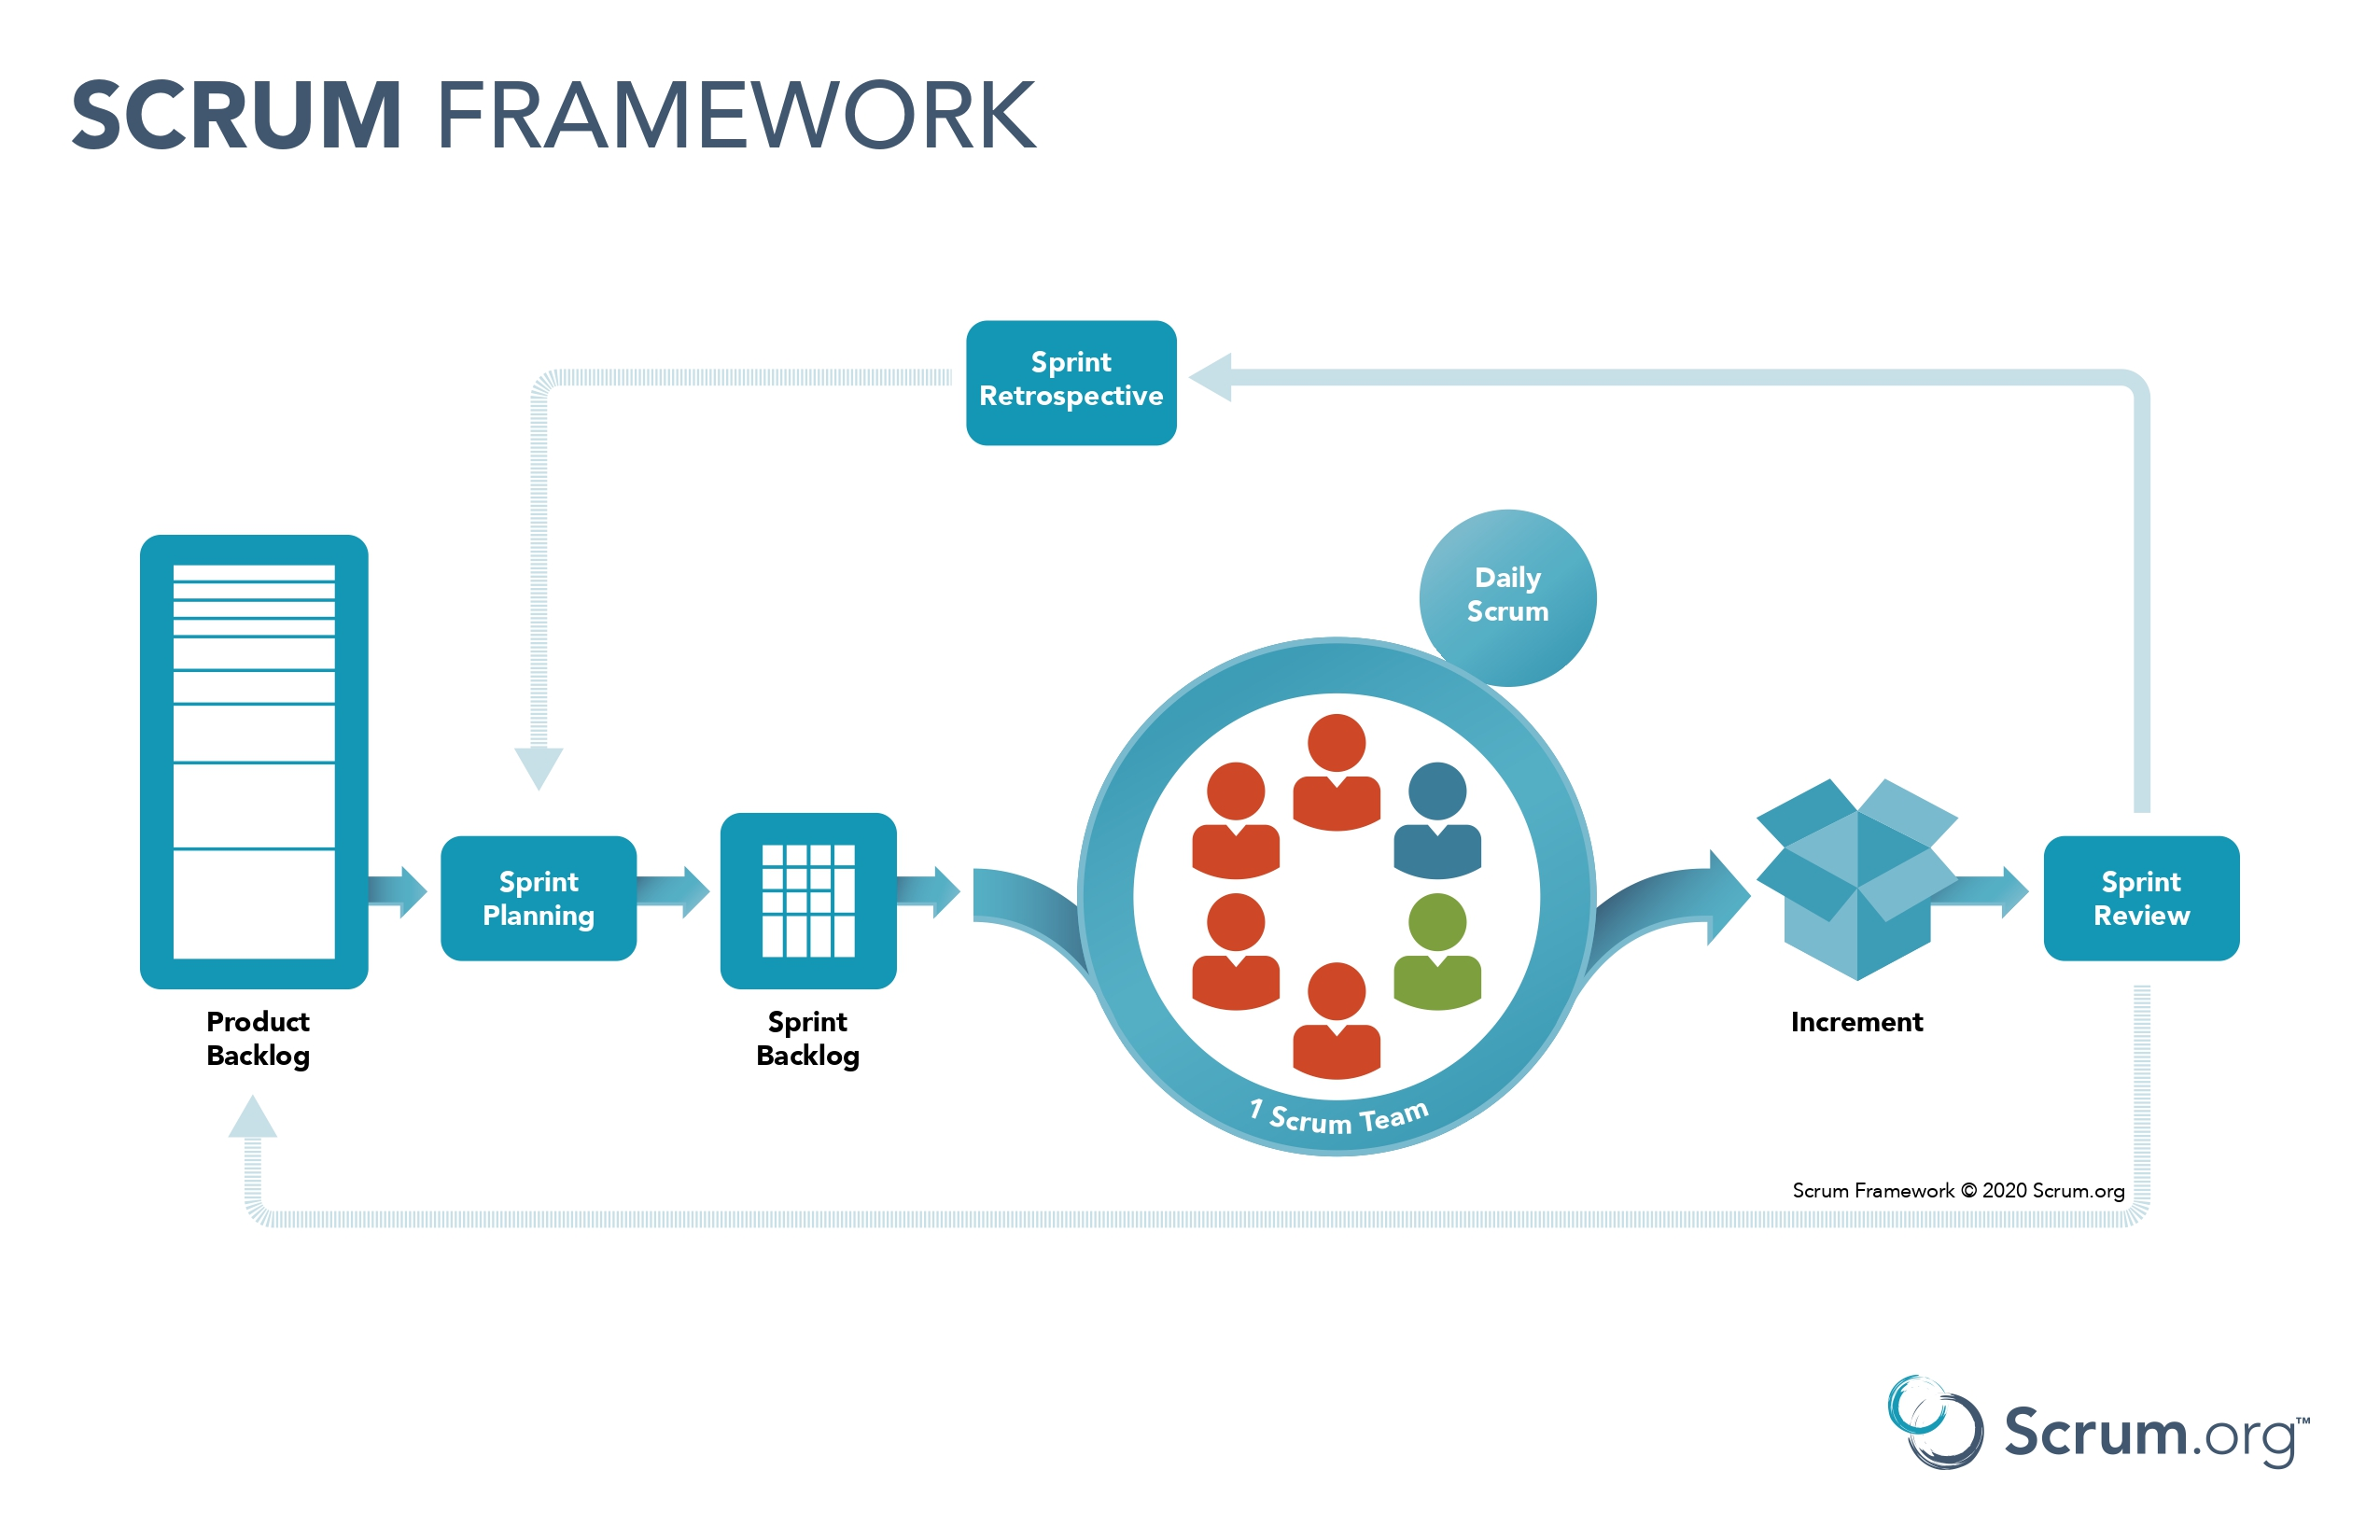
\includegraphics[scale=0.3]{scrum}
                \caption{Le cadre de travail SCRUM}
            \end{figure}
        Pour une implémentation réelle, le framework Scrum nécessite le regroupement et le respect d’un certain nombre d'éléments qui font sa particularité. Ce sont notamment:

        \begin{itemize}
            \item Les \textbf{piliers: } Scrum dispose de 3 grands piliers empiriques à savoir: la \textbf{transparence}, l' \textbf{inspection},  l'\textbf{adaptation}.
            \item Les \textbf{valeurs: }pour réussir bien un projet Scrum, les membres de l'équipe doivent être capables de respecter cinq valeurs fondamentales: l' \textbf{engagement} à suivre les objectifs fixés, le \textbf{focus} sur le but commun, l' \textbf{ouverture} face aux difficultés professionnelles, le \textbf{respect mutuel} entre les collaborateurs et enfin le \textbf{courage} pour une exécution de manière excellente des tâches et la relève des challenges.
            \item Les \textbf{événements: } 4 (quatres) événements majeurs permettant la création de la régularité font la méthodologie Scrum: les \textbf{Sprints} d'une durée fixe allant de 2 semaines à 1 mois au plus, le \textbf{Sprint Planning} qui lance un sprint, le \textbf{Daily Scrum} pour inspecter les progressions, le \textbf{Sprint Review} pour analyser les résultats et déterminer les adaptations futures.
            \item Les \textbf{artefacts: }ceux-ci représentent un travail ou une valeur. Nous avons trois artefacts Scrum: le \textbf{\textit{Product Backlog}} qui exprime l'objectif du produit, le \textbf{\textit{Sprint Backlog}} définit l'objectif du sprint et l' \textbf{\textit{Increment}} qui établit la signification d'un \textit{"sprint terminé ou fini"}.
            
            \item L' \textbf{équipe: }Scrum s'organise toujours autour d'une petite équipe d'au plus 10 (dix) personnes. Cette équipe est composée des \textbf{\textit{Developers}} qui implémentent concrétement chaque incrément d'un sprint, le \textbf{\textit{Product Owner}} qui détaille les objectifs du produit à livrer, le \textbf{\textit{Scrum Master}} qui met en place le Scrum et assure l'efficacité de l'équipe.
        \end{itemize}
    Pour ce qui concerne notre projet, notre Scrum Team était constituée comme suit:
        \begin{table}[H]
            \centering
            \begin{tabular}{|l|l|}
                \hline
                \rowcolor{Gray}
                \textbf{Fonction} & \textbf{Noms et Prénoms} \\ \hline
                \textbf{Product Owner} & \textbf{M. Youssef} \\ \hline
                \textbf{Scrum Master} & \textbf{M. Marouane GHOULAMI} \\ \hline
                \textbf{Developers} & \textbf{M. Hisdaele KAMGA} \\ \hline  
            \end{tabular}
            \caption{Scrum Team du projet}
        \end{table}
    Nous avons suivi des sprints d'une semaine. La définition des objectifs sont définies en début de semaine. À la fin de la semaine, un rapport sur le sprint achevé est effectué et contient l'état d'avancement du projet ainsi que les perspectives pour le prochain sprint.

    \subsection{Outils d'organisation et de communication}
        Toute équipe de projet doit savoir d’une part s’organiser et d’autre part communiquer. Avec l’essor de l’informatique, ces tâches essentielles deviennent plus faciles. En effet, il existe plusieurs plateformes gratuites qui permettent aussi bien de planifier et suivre les activités d’un projet que de faciliter la communication au sein de groupe de travail. Pour notre projet, nous avons opté pour des outils simples et largement connus:

        \begin{enumerate}
            \item \textbf{Trello: }lancé en \textbf{septembre 2011}, Trello est un outil en ligne de gestion de projet inspiré de la méthode Kanban de Toyota. Il repose sur une organisation des projets en planches listant des cartes, chacune représentant des tâches. Les cartes sont assignables à des utilisateurs et sont mobiles d'une planche à l'autre, traduisant leur avancement. Ainsi Trello va nous servir à représenter les différentes informations sur les sprints en cours, effectués.
            \item \textbf{TeamGantt: } pour pouvoir planifier les différentes tâches et les visualiser, nous avons utilisé le \textbf{diagramme de Gantt}. C'est un outil pour l'ordonnancement et la gestion de projet. Elle permet d'un coup d'oeil de \textbf{déterminer les dates de début et de fin des tâches}, d'\textbf{identifier les marges existantes sur certaines tâches} et de \textbf{connaître l'état d'avancement du projet en général}. Pour créer ce diagramme de Gantt pour notre projet, nous avons travaillé avec la plateforme en ligne TeamGantt. Elle permet facilement de placer de nouvelles tâches avec leurs dates de début et de fin sur un diagramme de Gantt.
            \item \textbf{Skype: }c'est un logiciel qui permet de faire des échanges téléphoniques, vidéo et des messages via internet. Nous l'avons utilisé au cours de notre projet pour échanger des messages et partager certains fichiers ou liens utiles pour l'avancement des travaux.
            \item \textbf{Microsoft OutLook: }c'est un gestionnaire d'informations personnelles et un client de courrier électronique propriétaire édité par Microsoft. Ce logiciel informatique fait partie de la suite bureautique Microsoft Office. Bien qu'il soit principalement utilisé en tant qu'application de courrier électronique, il propose aussi un calendrier et un gestionnaire de tâche et de contact. Nous avons utilisé ce logiciel pour communiquer officiellement avec le Product Owner et le Scrum Master. A travers cet outil, nous envoyons avec une certaine régularité les rapports d'avancement du projet avec les prochaines perspectives.
            \item \textbf{Microsoft OneNote: }pour les prises de notes importantes, nous avons opté pour Microsoft OneNote. C'est un programme développé par le géant Microsoft qui nous a permis de tracer les avancées journalières.
            \item \textbf{Google Meet: } c'est un outil de vidéoconférence développé par Google. Nous l'avons utilisé pour faire certaines rencontres de mise au point en ligne avec le Manager M. Youssef. 
        \end{enumerate}

        \begin{figure}[H]
            \begin{subfigure}{0.3\textwidth}
                \centering
                
\includegraphics[width=\textwidth]{trello.png}
                \caption{Trello}
            \end{subfigure}
            \hfill
            \begin{subfigure}{0.3\textwidth}
                \centering
                
\includegraphics[width=\textwidth]{teamgantt.jpg}
                \caption{TeamGantt}
            \end{subfigure}
            \hfill
            \begin{subfigure}{0.3\textwidth}
                \centering
                
\includegraphics[width=0.3\textwidth]{GoogleMeet}
                \caption{Google Meet}
            \end{subfigure}

            \begin{subfigure}{0.3\textwidth}
                \centering
                
\includegraphics[width=0.3\textwidth]{microsoftOutlook.png}
                \caption{Microsoft OutLook}
            \end{subfigure}
            \hfill
            \begin{subfigure}{0.3\textwidth}
                \centering
                
\includegraphics[width=0.3\textwidth]{oneNote.png}
                \caption{Microsoft OneNote}
            \end{subfigure}
            \hfill
            \begin{subfigure}{0.3\textwidth}
                \centering
                
\includegraphics[width=0.3\textwidth]{skype.png}
                \caption{Skype}
            \end{subfigure}
            

            \caption{Logos des outils d'organisation et de planification}
        \end{figure}


        





